\section{Introduction}
The degree to which a general purpose corpus represents ``real'' language use is often debated at length, and is the key issue affecting design of corpora.  A wide variety of methods have been used to estimate language proportions and usage for a whole population, however, these are mediated by (and often centre around), expert opinion.

Reasons for this approach are both theoretical and practical---sampling individuals in the act of using language is very difficult (something other social sciences also struggle with), and the persistent nature of texts means that they conceptually stand alone, especially where the corpus designers intend to include older works.

Nonetheless, there is a missing empirical link between the expert-guided designs of language proportions and the ground truth of an individual's language use.  This is lamented by many who wish to study language acquisition (or more detailed explanatory theories regarding language use over time \td{cite Hoey, quote too}.

This chapter describes a case study whereby a census of text types was attempted for a single individual.  This sample design yields very little inferential power regarding the whole population, but serves to illustrate the disparity between the proportions a general purpose corpus may have, and the language used by an example individual.  The extent to which this example individual may be a useful guide for corpus building is not addressed directly, but this is an area that could be expanded using demographic auxiliary data.















% ============================================================================
\section{Sample Design}
As we have seen in chapters~\ref{}\td{ref}, conventional corpus building efforts centre around linguistic variables, and rely largely on expert opinion to balance their socioeconomic variables.  This approach was initially selected in order to avoid certain practical problems (many of them caused by technological limitations), though it has also caused others, most notably the difficulty in retrieving metadata about texts post-hoc.

Often, the only way to ensure demographic balance is to rely on sources of auxiliary data such as bestseller lists and library loan records that map textual variables to socioeconomic ones.  This process of using `proxy' variables is particularly opaque, and often limits the metadata available.

The intent of this chapter is to sample in an ad-hoc manner, that is, to record details of a text or single use of language in context, as it is used.  This approach is far closer to that used in special purpose corpora, especially where the restricted domain allows use of automated recording tools or sampling from an existing rich database (such as from an online forum).

The case study itself takes the form of a census of language use, for a given period, for a given person.  This offers empirical validity for linguistic proportions, but is a single data point from the population of language users and cannot be formally generalised.

Of particular interest are variables that are particularly challenging to sample:

\begin{itemize}
    \item The age of a text when ``used''
    \item Other temporal information, such as the times and days when texts are read, and inter-day variance etc.
    \item The social context of text use
    \item Attention paid to a text, and which portions were read
    \item Proportions of text types used, especially representation of types that may be missing from other corpora such as greetings, billboards, product labels.
\end{itemize}

The ad-hoc sampling approach, applied to \textsl{all} texts used, also allows inspection of the proportions of language types used---something that is estimated for general purpose corpora.  Though the scope of this case study is necessarily limited, a ``language use census'' for many people would be a robust empirical method for validating claims of representativeness in GP corpora.


A further advantage of this method is that the population may be rigorously defined, as data on the participants is available to whatever standard deemed necessary.  This is notably at odds with the use of existing lists or repositories, which have been constructed with differing purposes and levels of documentation.






\subsection{Difficulties and Disadvantages}
Sampling language use ad-hoc involves changes in sampling strategy that are practically challenging.  Taking this study as an example, one would have to take data from enough people to cover the population required, and each would have to undertake a fairly in-depth procedure.

Difficulties encountered when trying to sample large populations are well documented in the social sciences, and many techniques exist to mitigate common biases (\td{such as}), however, these are largely beyond the scope of this chapter.  It is notable that one solution in sociology has been to share data (in a style similar to corpus linguistics) in order to minimise the costs involved in implementing a high quality survey.

The increased ``person-focused''ness of a primarily social design also raises a number of ethical issues, as it is increasingly possible to derive information not just about a general group's language preferences, but about an individual's (or a comparison between groups).  This is merely the inverse of its value, but it is nonetheless worth considering as many study designs in linguistics need not work with such sensitive data.  This issue is addressed after the discussion of methods and findings\td{Ensure that it is.}.

Further, sampling text as it is used raises methodological challenges---how can we be sure that the language observed is still naturally occurring and valid?  All sampling is going to compromise on this, and the extent to which one values detail over interruption will vary by study design.  The aims of this study are, in part, to identify major challenges in this area, for example, which text types are most difficult to sample or require most time to record.














% ============================================================================
\section{Technology}
As mentioned, a number of the limitations to this kind of sampling may be addressed through the application of new and emerging technologies.  This takes two main forms:

\begin{itemize}
    \item Many more documents are now poduced and consumed in digital form.  This means they are accessible for automatic copying and processing by sampling software, often without any intervention necessary by the user.
    \item The abundance and ubiquity of portable technology such as smartphones lowers the difficulty of many existing sampling methods such as audio recording or photography.
\end{itemize}


The former of these is well represented by the WaC movement in corpus linguistics, and many corpora include sections which have been sampled by distributing portable technology\til{So, er, this is where the lit review seems out of place 'cause it's in chapter 2}.  Of particular interest, however, is the value that we may extract by exploiting both to form a coherent narrative.

One community that has been using these techniques extensively is that associated with life-logging.  Life-loggers do stuff---see lit review.










\subsection{Life Logging}
Just as the availability of portable recording technology made acquisition of spoken corpora relatively easy to control, so have the limitations on digitisation and format conversion limited the selection of written text to those already-indexed properties.  As modern computing devices have miniturised and become ubiquitous, they have developed a number of capacities that may be used to afford the same ``instantly recordable'' status to non-spoken language use.


A number of these technologies are as a direct result of the life-logging community's interest in multimedia records.  Life logging is an activity that emerged slowly out of the principles of webcam shows and reality TV.  It involves recording (and usually broadcasting) continuous information about one's life as it occurs.

Though most popular efforts started as a means for providing entertainment, and thus focused on multimedia broadcasting on the web, the techniques required soon diversified and gained the interest of the information retrieval and processing communities.  Many projects have been started with an aim to catalogue and operationalise the huge stream of data each person creates, largely with a focus on aiding that person in their daily life, or aiding large organisations (such as defence forces) in management of resources and people.

\til{citations and a proper lit review, but they are maybe better off elsewhere}

Because of the continuous nature of life-logging, many efforts have been made to use methods that are easy to maintain, self-contained, and covert.  % CITE
Due to this, as well as the original intent of the life-logging process, much of the effort surrounding life-logging focuses on multi-media sources, and how they may be best combined to form a coherent idea of context.  

Typical sources of data considered include:

\begin{itemizeTitle}
    \item[Video recording] Many life-loggers wear systems that are able to continuously record video in the direction they look, and upload this using mobile networking systems.
    \item[Audio recording] Due to its lower obtrusivity, many efforts surround the analysis of audio logs, and include systems to detect voices and identify events such as making appointments.
    \item[Document storage] With the increase in use of digital-origin documents, some of the more holistic life-logging systems record documents as they are read, with a focus being to integrate this data into the larger picture.  Others scan in their post for later retrieval.
\end{itemizeTitle}

Many of the requirements of a life-logging platform (covert operation, comprehensive data management, context identification) overlap notably with the methods used in covert sociological research and, of particular note for our purposes, those constructing spoken language corpora.

Notably, one of the methods used to create the spoken portion of the BNC was covert recording, where a number of people were provided with tape recorders...
\til{ Quote from BNC documentation }

As illustrated by the BNC's demographic balancing of that portion of their corpus, this ability to directly record data from the field satisfies the disadvantages of text-index-oriented methods of document selection, allowing us access to all of the contextual data at the time of text consumption/production 
\til{perhaps because the time of production and consumption don't differ much for spoken stuff...}

The cost of this is, as felt by all sociological studies, a need to find a sufficiently large and heterogenous sample of people who may record data about their language use (and for long enough for it to be useful to researchers).  This is arguably more difficult in practice than text-index-based methods, and should only be considered at a large scale where the difference is likely to be crucial to a study, nonetheless, large samples exist in sociology as testament to the value such designs may yield [and the illustration that no alternative method exists for many sociological issues].

The benefit of having a clearly-defined population about which to generalise linguistic findings is applicable to any size sample, however, making techniques of logging particularly applicable to special-purpose corpora, especially where those corpora are best demarcked along social lines.  Indeed, at one extreme of this scale exists the concept of a personal corpus; something that may yield insights or models about a single person's current language usage.  Such a resource may one day be particularly valuable in defining how one uses text-based interactive systems (such as the web), reads content (such as news articles) or even how one would learn.

Such designs exhibit a tradeoff: a decrease in socioeconomic breadth in exchange for an increase in linguistic breadth.  It is my intent to illustrate the value in this approach, and to investigate methods by which it is possible to construct corpora without undue difficulty through the use of life-logging methods.
% This needs mega elucidation, methinks



\til{ Intro to life logging, a good lit review needs to be done.  Perhaps it belongs in the lit review section rather than here though.}

















% ============================================================================
\section{Approach \& RQs}
The case study described here is an attempt to assess the extent to which techniques from life-logging may assist corpus builders in creasing a demographically-oriented corpus.

It follows an iterative design surrounding these aims, with each iteration refining a number of key design areas:

\begin{itemize}
    \item The variables that may practically be recorded about a text (and that must be before they are lost);
    \item Methods that may be used to sample text unobtrusively, especially how new technologies may be used to assist;
    \item Methods and tools for operationalising logs after sampling is complete, and how these may assist the process of data gathering itself.
\end{itemize}
\til{I'm sure I'm missing stuff here.  Check notes and presentations}

Ultimately, the differences in sample design contribute to a larger picture that could yield much future work.  The direct research questions addressed here are:

\begin{itemize}
    \item What methods may be used for gathering data in a short-term language census?
    \item How may the collected data be operationalised?
    \item What proportions of language are used by the subject; do these support common claims from general purpose corpora?
    \item How may these methods be used in future to aid those building corpora?
\end{itemize}







\subsection{Sampling Policy}
\label{sec:personal:samplingpolicy}
\td{from notes}
The aim of a personal corpus is to emulate, as closely as possible, a census of observed language.

Use of language, in this context, is defined as any conveyance of information, spoken or written, in any quantity. There are no bounds to the context in which it is used, nor the language itself, as the purpose of the study is to evaluate these very things.

Each of these transactions is recorded as a single line in the data set, and will be annotated with the variables recorded.  One of the major issues encountered in preliminary tests was annotation for attention and proportions read.  These will be recorded along with textual properties to ease operationalisation.

Attempts were also made to record sufficient data to retrieve the full text of each transaction.  This worked better for some data sources, and much of the case study thus concerns itself with (sometimes estimated) word counts.  Word counts were chosen as a measure of size due to their use in other corpora, and their applicability to many different media.


A number of practical challenges were identified before sampling, and these were backed up by experience:
\begin{itemizeTitle}
    \item[Review and Production] Both should be recorded as fully as possible. Where a text is re-read, or developed and continually re-read, this should be noted as an ongoing process (and accordingly oversampled).
    \item[Short Utterances] Very short interactions, such as passing greetings, should not be under-recorded. Their inclusion is likely to be one major difference from conventional corpora.
    \item[Oft-reread Texts] such as labels, signs and the like. It’s debatable whether or not one actually reads or merely remembers/recognises these. Perhaps psychological literature (Gestalt, etc.) can shed some light on this?
% See Wang, Zhe, and Gemmell, Jim, Clean Living: Eliminating Near-Duplicates in Lifetime Personal Storage, Microsoft Research Technical Report MSR-TR-2006-30, March 2006.
\end{itemizeTitle}










% ============================================================================
\section{Method}
As mentioned in~\ref{sec:personal:samplingpolicy}, the primary objective of the sampling is to record all ``linguistic events'' for a given period, for a given subject.

The subject chosen was myself---this was done for a number of reasons:

Firstly, legal and ethical issues surrounding recording and review of the data were mitigated by having the analysis performed by a member of the original conversations, etc.

Secondly, iterative review of methods involved was possible with internal, `white box' examination of how data were collected, and what edge cases and procedural difficulties arose.

Thirdly, the demographic status and other person-related variables are well known and need no formal elicitation, minimising time spent on construction of questionnaires et al.


\subsection{Data Sources}
Before the first iteration of the sampling/review process, all of the possible language data sources used in everyday life of the subject were informally identified.  It soon became clear that these data sources exhibited properties that would make sampling easier, or less intrusive.  They were classified by the methods required to capture their text:

\begin{itemizeTitle}
    \item[Persistent] Resources that exist in a format that is easily retrieved and immutable.  This covers many physical items such as books, and some broadcast media as well as notes made in a notebook.  Only identifying information must be stored during sampling itself, in some cases merely an ISBN or similar index code.
    \item[Ephemeral] Language data that cannot be accessed after-the-fact in any way, or may differ by time or context.  This most obviously contains speech, but also many websites, things such as billboards that cannot be readily re-accessed, or todo lists that get destroyed.
    \item[Digital Origin] Documents that are read, or written, on electronic devices.  These may fall into either of the above categories, yet they may usually be copied with no overhead so it is often simpler to store them at the time of use.  Many document types are now digital, as well as the obvious sources such as email or online chat.
\end{itemizeTitle}

This classification was useful in order to minimise the intrusiveness of a collection method, whilst maximising the detail recorded for a given source (ideally to the point of storing verbatim text).  In practice, methods were easy to develop for automated recording of digital documents, and many techniques exist for sampling non-digital persistent and ephemeral sources with scientific levels of accuracy already.

The sources identified in the initial case study were as follows:

\td{Merge these two lists with a separator or something?}
\begin{itemize}
    \item Speech
    \item Printed documents (i.e.\ letters, brochures)
    \item Digital documents (same, but unprinted)
    \item Terminal logs
    \item IRC logs
    \item Email
    \item Websites
    \item Unusually formatted printed material (posters, labels, advertising on vehicles, billboards, etc.)
\end{itemize}

The inadequacies of introspective methods to identify these soon became apparent during preliminary tests, as the process of recording increased awareness of language use, raising a series of edge cases.  These were collected and resulted in a final selection of sources displayed below.  As well as expending the set of sources to be gathered, methods of collection were chosen with flexibility in mind in order to cope with unenvisaged sources of data\footnote{This flexibility has the unwelcome effect of slowing down analysis later on, and may be undesirable in some cases}.


\td{This image is complete, but not in the git repo.}
\begin{figure}[p]
\centering
% \includegraphics[width=0.4\textwidth]{datasources}

\includegraphics[width=0.4\textwidth]{missing}
\caption{Data sources and their appropriate capture methods}
\label{fig:personal:datasources}
\end{figure}



\begin{itemize}
    \item Speech
    \item Printed documents (i.e.\ letters, brochures)
    \item Digital documents (same, but unprinted)
    \item Terminal logs
    \item IRC logs
    \item Email
    \item Websites
    \item Unusually formatted printed material (posters, labels, advertising on vehicles, billboards, etc.)
    %---
    \item Written (but non-OCRable) material
    \item Key strokes
    \item SMS records
    \item Phone conversations (separated from speech as they yield differing metadata)
    \item Music tracks
    \item Files accessed
\end{itemize}

This list is necessarily furnished according to the life of the subject in question---from this study I am unable to assert that it is generalisable to others, though the process of doing so would involve relatively little intrusive sampling\td{link to further work}.

Each of these sources is ``covered'' by one or more sampling tools.  These tools progressed most during the iterative process, and each was subject to a number of procedural subtleties that were refined throughout the study.


\til{Diagram from notebook, figure~\ref{fig:personal:datasources}}










\subsection{Recording Methods}
Recording methods were chosen for a variety of reasons.  First and foremost they must, in sum, cover the sources mentioned above.  Secondly, they were selected in order to be unobtrusive both for the experimenter and those around him.  Thirdly, they were selected to be flexible enough to cover unforseen contexts and data sources.

The methods used can be separated further into two groups: many methods are capable of recording multiple sources, and serve to form a narrative that describes the metadata of a linguistic event, pointing at another source for the data itself.  These methods were chosen to allow for post-hoc ``memory jogging'' and narrative creation, something that was added to the experimental procedure after the first iteration indicated how difficult to operationalise much of the data would be.

The second set of methods are focused on a single data source, typically requiring little to no manual intervention to record it.  Their records are either indexed by time, or by the more flexible methods mentioned above.


\subsubsection{Indexing and Overview}
\paragraph{Journals and Note-taking}

\begin{figure}[p]
\centering
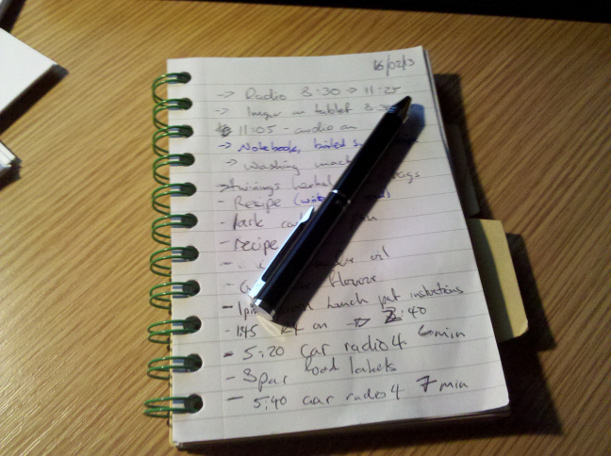
\includegraphics[width=0.8\textwidth]{notebook}
\caption{The `on-line' notebook}
\label{fig:personal:online_notebook}
\end{figure}

Two journals were maintained throughout the sample.  The former of these was an A6 notebook maintained `on-line'\td{rename to hot/warm/cold, front/mid/backline or something similar} as events occurred (pictured in figure~\ref{fig:personal:online_notebook}).  This was used to store durations of conversations, titles of persistent sources, etc.

The second was an off-line journal, maintained at the end of each day in a narrative style.  This blog-like record was intended to reflect in depth on the proportions of text used in each source, and how attentively each linguistic event was engaged in.  The writing of the journal itself was not logged by any other methods.  It was also possible to attach daily records to this journal, and the process of writing it inserted an opportunity to reflect on the mnemonic codes used during the day.  This process is described in context in section~\ref{sec:personal:recording}.

The on-line notebook proved to be the primary indexing method for all other sources of data, and its maintenance was the primary overhead of the study.  Each entry in the notebook was eventually reduced to a compressed form that roughly followed one-line-per-event, storing the time each event occurred, any identifying information deemed necessary for later memory of it, and a duration or other index of word counts.

\til{Insert a picture of one of the scanned days, pointing out the format}

Problems of simultaneous events and split attention were solved in the notes by having a start/stop event for ongoing events, and by using the off-line journal to reflect upon each event.


\paragraph{Audio Recording}
Following work on machine listening, the original intent of audio recording was to capture the occurrence and duration of conversations, as well as any smaller interactions that would otherwise be difficult to capture (such as greetings, thanks when opening doors, etc.)


\begin{figure}[p]
\centering
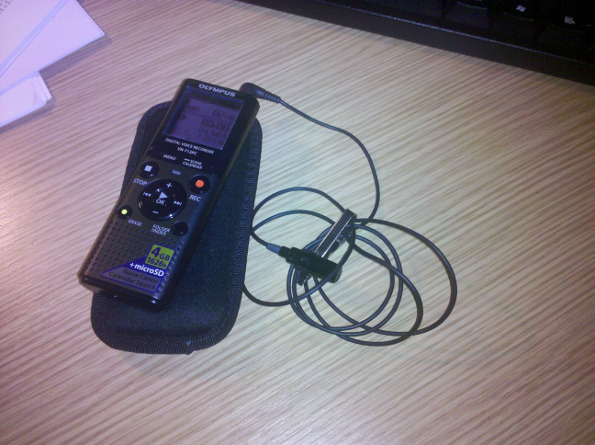
\includegraphics[width=0.8\textwidth]{dictaphone}
\caption{The audio recorder used}
\label{fig:personal:audiorecorder}
\end{figure}



Capturing was performed with an Olympus 713PC\td{check this, is it PC713?} dictaphone, recording to a suitably sized external card that yielded many days' continuous recording.  Provision was made to download recordings each night and store them with the off-line journal, however, in practice they remained on the recorder until the end of the study.


\begin{figure}[p]
\centering
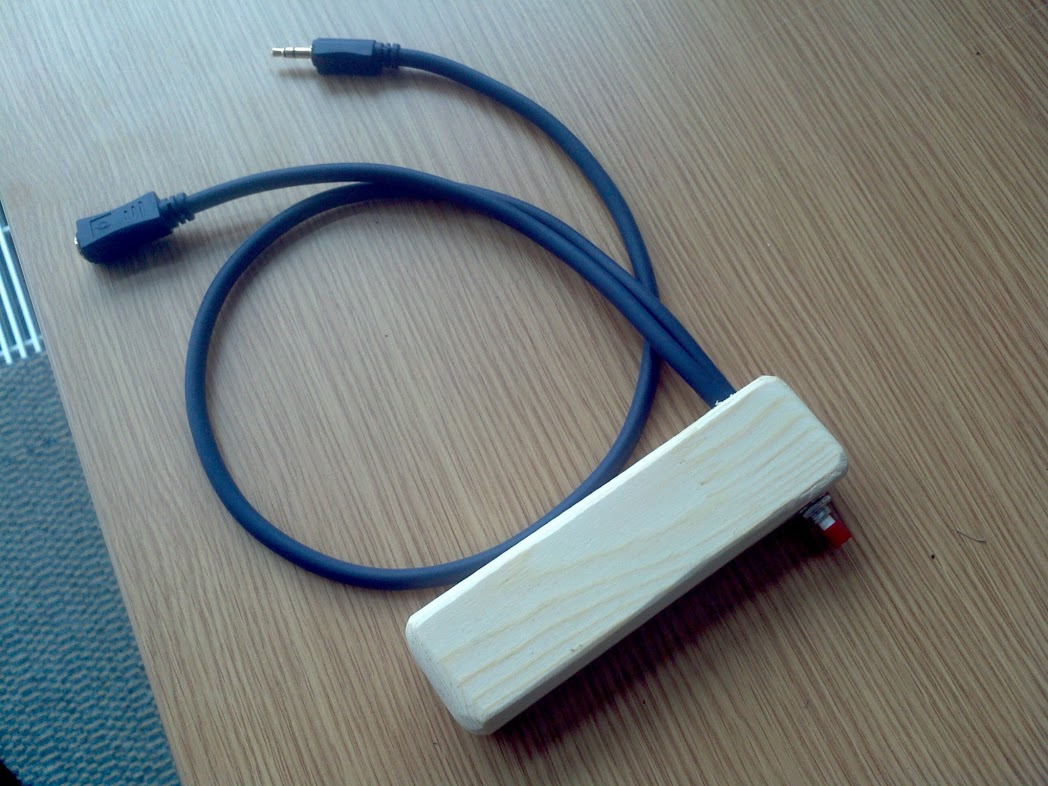
\includegraphics[width=0.8\textwidth]{clicker}
\caption{The second audio index marker}
\label{fig:personal:clicker}
\end{figure}


Aligning the recorder's output to the events mentioned in the notebook was a tricky process---Though the recorder itself supports index marks, there is a limit of 99, which was deemed riskily low.  Two devices were built to insert absolute silence onto the recording (something that is rare in real life and easy to programmatically detect), the later of which is pictured in figure~\ref{fig:personal:clicker}.  These clickers were to be pressed at the beginning of each conversation, so that voice activity detection could be performed to estimate the word count of each conversation (or, in an ideal world, extract verbatim text).

In practice, the process of tapping the button proved intrusive and, from the perspective of one talking to the subject, suspicious.

The mechanism used for the final iteration of the study was far simpler---the recorder's start time was written in the on-line notebook, and entries therein were keyed by computing the offset between the two times.  Though this incurs a minor overhead in coding the data, it also allows for spontaneous conversations without much overhead, something that is particularly important to the study of text type proportions.



\paragraph{Photographs}
The primary method of capturing ephemeral, irregularly formatted, non-digital texts was photography using a cameraphone.  This method was chosen largely because the ubiquity of smartphones in British society has led to a situation where photographing fairly mundane items is widely unquestioned.

The smartphone used, a Motorola Milestone, also stores time and location data in its photographs using EXIF tags (as well as storing photographs sorted by day).  This metadata meant that there was often no need to file an entry in the on-line notebook, and the cameraphone could simply be used in a very unobtrusive ad-hoc manner.

In earlier iterations of the study, it became apparent that the loud shutter noise made by the Android operating system when taking photographs was problematic.  Though photography of signs, packets and such remained unchallenged, the attention of people nearby was drawn to the weirdo with the cameraphone all too readily.  This was solved partially by (with great difficulty) disabling the noise, though it was still apparent from posture when a photograph was being taken.

There are notably a number of products available that continually take photographs for the purposes of life logging.  These were considered for the study, but their aims are generally to capture each event, rather than specific aspects of selected scenarios.  The ability to consciously specify that the subject was more attentive in some situations (and take pictures accordingly) was judged to outweigh the value of having a continuous record (something much more capably performed by the journals).




\subsubsection{Targeted Methods}
\paragraph{Phone Calls \& SMS Messages}
Both of these are automatically logged by the Android operating system used by the subject, and each was also indexed in the on-line notebook.  The data was extracted using a free application that exported to XML.


\paragraph{IRC}
IRC was logged by construction of a bot.  This bot accompanies the subject into chatrooms and logs all messages observed, applying a rough human interest model to ignore data seen when the user is set to away.


\paragraph{Web}
The SQUID webproxy was configured to log all traffic, and a number of logins were provided---one for each of the subject's internet-enabled devices.

The logs from SQUID store all requests, including advertising/tracking calls, downloading of things never read by the user (i.e. CSS and Javascript) and AJAX calls to partially reload pages.  As such, a large amount of processing was necessary to extract URLs from these logs, and to parse the resultant data into a usable format.

\paragraph{Keylogging/Terminal recording}
Terminals and keyboard input were logged using a custom application that wrapped a terminal, recording the time each character was sent or received to the shell.

Each terminal created started recording to a new log file, storing the time at which it was started and a series of offsets from this time.

\paragraph{Last.fm}
In earlier iterations it was apparent that lyrics in music were being missed as a source of text---all devices capable of playing music were configured to `scrobble' to the last.fm music service during the sampling period.

Though last.fm do not make their data freely available for access, third party tools exist to scrape their website and download detailed logs of tracks listened to.

\paragraph{Files}
Files were identified in a number of ways.

Some, particularly those on which the subject worked and contributed data, were written down in the journals.  This is a precise method of separating what has been read, but might require a large overhead.

Since the subject works entirely on projects and files that reside in a RCS repository, the logs from each commit were used to generate a diff, and this was accessed after the sampling period to identify contributions made.

Another policy that may be used is identification of files by unix mtime (modification) or ctime (creation), however, this is fraught with inaccuracy, as files are liable to be modified on disk many times whilst being edited, and sampling the differences is likely to happen at haphazard times.  Further, this technique would capture many log files and others that have been edited by processes where the subject was not involved linguistically.  By contrast, commits to an RCS are scheduled around logical additions, and are manually pushed so that only deliberately edited files are stored.

Files uploaded whilst on other systems may be uploaded directly to the off-line journal (which, ironically, is online), or stored on a flash drive that was carried specifically for the purpose.  In practice this did not occur during the recording period, though experience suggests these contingencies would be necessary if a longer sample were taken.

\paragraph{Email}
Emails are, again, stored automatically with sufficient metadata as to make them self-documenting.  However, rather than presume all were read in a given day, each was tagged after being read with a label corresponding to the day.

At the end of the sampling period, these tags were collected and downloaded in mbox format, whence they were processed by the operationalisation script.









\subsection{Recording Procedure}
\label{sec:personal:recording}
The study is based around a period of continuous sampling using the methods discussed above.  For two weeks (in some cases longer), data was captured for each source.  This process was structured around a daily routine:

Upon waking, and before any language was used, the recorder was turned on and a note of the time at which this occurred was made in the on-line notebook.  Recording was then continued until the end of the day without interruption.

The on-line notebook, smartphone, and flash drive, were carried at all times.  Since each of these could be backed up (the smartphone even did this backup automatically), the most data at risk was a single day.

Notebook entries were made as soon as was possible without interrupting the linguistic event being recorded.

At the end of the day (immediately prior to sleep), a journal entry was written in the off-line journal, and SQUID logs were uploaded for the day.  This journal entry forms a narrative, estimating the time taken and attention paid to items in the on-line journal for that day, as well as detailing anything that may be written in shorthand-mnemonic form.










\subsection{Operationalisation, Processing and Analysis}
Normalising and operationalising such heterogenous data without significant overhead proved to be a significant problem that was only partially solved, and the data set presented here required significant manual intervention that was possible in part due to the fact that the analyst was the subject.

This advantage, clearly, cannot be relied upon in other studies, and this part of the method demands most further study in order to define typical parameters for many processes that are dependent on human properties.

Two main processes were followed in data processing.  The former of these was aggregation and normalisation---each data source was collected and transformed into a one-event-per-line CSV containing a standard set of fields (the selection of fields used was modelled on Lee's BNC index\td{CITE} in order to facilitate comparison).

After this normalisation process was complete, data were manually annotated to complete any fields that were not stored in the original metadata.  This was largely an objective, uncreative task that simply demanded human reasoning capacity, but it is inevitable that some bias will creep in at this stage.

The second stage of processing involved coding text types and roles.  This task is altogether more flexible and subject to design errors and bias than many of the normalisation stages, and was thus attempted in a manner that was designed beforehand.  Since the aim of this study is, in part, to identify text types not seen in other corpora, following an existing taxonomy would necessarily limit the coding of any newly discovered.  True free coding, however, is likely to draw distinctions between text types that are not made in existing taxonomies, rendering them incomparable.

The process followed was a hybrid approach---data were freely coded by inspection of the texts, but this was done with deliberate prior knowledge of Lee's classification scheme.  The intent was to categorise texts according to Lee's scheme only in so far as they were deemed suitable by the analyst (who is also, lest we forget, the subject).

Though this approach was suitable for the aims of this particular study, it is difficult to advocate for any others using the sampling techniques described, and its use here should not be taken as such.

%---
\subsubsection{Human Interest Models}
Beyond coding, by far the largest single influence on the data recorded was the human interest model applied.  This was created in order to take into account two factors that had become particularly apparent (and notably do not apply in the same manner to conventional corpus designs, where many eyes may cover a whole document in sum):

\begin{itemize}
    \item Often, only small (usually predictable) portions of a text are used.  For example, I have started to read more books than I have finished reading.  Generalised, this means that even Brown-designed corpora should favour the start of their texts slightly when selecting excerpts.  Some media were more surceptible to this than others, and the automated normalisation tools were built with facilities to take this into account.
    \item Texts, especially broadcast media and speech, were often used whilst also accomplishing a non-textual task (or sometimes both at once, such as talking with the radio on in the background).
\end{itemize}

Both of these were noted in journals, and added to the processing toolchain---each data source's normalisation script contained a model to extract the portions of text that were read, and each row of the normalised data format contained an ``attention index'', ranging from 0--1, that served as a coefficient of the word count.

Though crude, this measure was able to produce approximations for word counts that were inline with the expectations of the subject.  (It is recognised that this may not hold much scientific value to others wishing to replicate the study, and in general it is necessary to investigate the inter-person variability of these properties in order to create more generalised processing tools.)


% TODO: perhaps a run-down of each annotation program?
\paragraph{Web logs}
The human interest model for web logging was built by inspection of the web logs and cross-referencing with information about the hosts identified.  The normalisation script is concerned primarily with removing material that was downloaded without ever having been viewed, for example, non-text MIME types and advertising, and contains a multi-stage strategy for excluding content:

\begin{enumerate}
    \item Filter only successful requests
    \item Filter only those requests that are of textual mime types (\texttt{text/*})
    \item Apply a blacklist of advertising websites and file extensions (manually constructed)
    \item Discard links where the page was reloaded and the URL is the same as the previous entry in the list (this pattern is often caused by initially connecting to the proxy, for example)
    \item Non-visible text items were discarded (non-body elements if the file is HTML), and markup was removed
\end{enumerate}

Beyond this initial normalisation, a speadsheet's \texttt{LOOKUP} function was used to manually assign attention coefficients to the domains, based upon entries in the journals and interesting portions of web pages that follow regular structures.

Days were classified as changing at 4am, since there were no points in the data set where the subject was still using the web at this time.



\paragraph{IRC Logs}
IRC logs were already stored using a limited attention model, which was based on the principle that, in IRC, conversations are started, live for a short time, then die off as people in the channel return to work.  The bot performing logging would start logging (and continue to log) for as long as the subject was talking, stopping 10 minutes after the final utterance.

In order to capture a human notion of day, that is, one demarked by sleep rather than midnight, the start time of each conversation was used to determine the day its data fell into.



\paragraph{Terminal [Console] logs}
Terminal data was logged with timestamps on each individual character, and the model was thus responsible for inferring when a command had output, and suggesting which portions of text were still on screen.

This was done with a `timeout' and a `scrollback'---the former describing a delay that had to be present for the text to have been read (rather than simply scrolling offscreen), and the latter describing the average size of a terminal (and thus the number of rows of text that remain displayed).

These parameters were tuned to match the specific data sampled over the period---for example, the time recorded included terminal use displaying logs from software that was being developed, and these would produce thousands of lines of output before a pause.




\subsection{Coding and Genres}
Since the case study is, in part, aiming to identify genre distinctions not found in other general-purpose corpora it is not possible to use an existing taxonomy to code text genres.

\til{Also note how I'm coding things from both spoken and written, and such, thus one taxonomy would be unable to cover it anyway?}


Genre distinctions were made using a process that loosely follows the principles of the coding stages of grounded theory \td{cite}.  
This involves a focus on free coding, and a consideration of all available context and information---something aided both by the `memoing' innate in the design of the journals, and the fact that the analyst is also the subject.  Free coding was performed with prior knowledge of Lee's genre categories.


This process was done in order to deliberately apply distinctions made by Lee to the data gathered, such that genres selected would be more easily compared to the BNC.  No effort was made to adhere to Lee's specification directly, as this would lead to over-specification where the case study's corpus proves more diverse in form than the equivalent BNC category.

It's particularly noteworthy here that the analyst selecting codes for genres is the same person as the subject gathering the data.  This, along with the mnemonic form of the notebooks and data captured, provides extra (informal) insight afforded by context.




% \paragraph{}





\section{Results}

\begin{figure}[p]
\centering
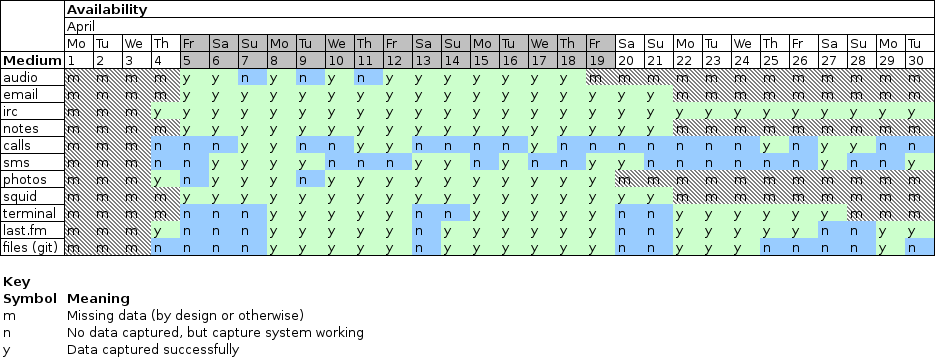
\includegraphics[width=0.8\textwidth]{dataoverview}
\caption{The availability of data from various sources}
\label{fig:personal:dataoverview}
\end{figure}


These results describe data collected during the third iteration of sampling, which lasted roughly two weeks during April 2013.  Table~\ref{figure:personal:dataoverview}\td{make into a table} describes the availability of data per-day.

The period marked from Friday the 5th to Friday the 19th (inclusive) forms the sampling period described herein (with exceptions to this noted where made).  This was the period for which the on-line notebook was maintained along with other intrusive data collection techniques, though notably some methods continued due to their ease-of-use.

Though audio data is missing for Friday 19th, this was not used due to the difficulty in processing such data ethically and within a reasonable time frame.  Word counts for spoken transactions were instead based on an estimated words-per-minute.  /%XXX: revisit this and do manual transcription some day before the viva?

This fifteen-day recording period covers 8,619 linguistic events, encompassing an estimated 980,000 words.  



\subsection{Variables}
Variables recorded on each linguistic event are based heavily on Lee's BNC index, augmented to take into account the attention index and word count estimates.  A summary of these is provided in Table~\ref{table:personal:variables}.

\begin{table}[hp]
\centering
    \begin{tabular}{ | l | c | p{7cm} |}
    \hline
    \textbf{Variable} & \textbf{Complete?} & \textbf{Description} \\ \hline
   
    source              & yes & The data source (email, audio, etc.) \\ \hline
    source2             & no & Any origin data from within the source (i.e. the caller in a phone conversation, sender for email) \\ \hline
    day                 & yes & Day of the month sampled \\ \hline
    mode                & yes & Spoken or Written \\ \hline
    circulation status  & yes & Exact circulation, or `h', `m', `l' following Lee's guidelines\\ \hline
    portion read        & yes & The attention index mentioned above \\ \hline
    informal genre      & yes & Free-coded genre \\ \hline
    medium              & yes & The form of the language used.  Usually the same as the source. \\ \hline
    % ...
    title               & yes & The title of the document, or an identifier for the text \\ \hline
    author              & no & The author[s] of the text\\ \hline
    author age          & no & The age of the author[s] \\ \hline
    author sex          & no & The sex of the author[s] \\ \hline
    author type         & yes & An indication of the type of entity authoring the text.  Follow's Lee's coding for \textbf{s}ingle, \textbf{m}ultiple, and \textbf{c}ommercial\\ \hline
    produced/consumed   & yes & During the transaction, was text produced, consumed, or engaged in interactively \\ \hline 
    % \hline
    words               & no & Authoritative word count\\ \hline
    duration            & no & Authoritative duration for spoken data\\ \hline
    computed words      & yes & Estimated word count, merging durations and word counts above\\ \hline
    computed genre      & yes & A composite of the medium and the informal genre, intended as a more specific genre representation \\
    \hline
    \end{tabular}
\caption{A summary of variables sampled}
\label{table:personal:variables}
\end{table}











\subsection{Activities}
During the sampling period, all work surrounding the personal corpus case study was stopped, in favour of other, ongoing, projects.  Other than this intervention, work continued as normal, which for this period involved significant amounts of development on the LWAC downloader tool.

% TODO: more about genera life in that period









\subsection{Frequencies and Summaries}
As mentioned above, the data collected constitutes roughly 9000 linguistic events, covering almost a million words.  In total 3.4GB of data were collected, though the majority of this figure (2.3GB, 67\%) of this is audio data which could easily be compressed or discarded after processing.

The overall word count is changed massively by disabling the attention model, rising to roughly 5 million words.  As we shall see later, this is largely because the data sources and genres which dominate the data set are particularly heavily adjusted.  This raises the question of how we may ensure accuracy of attention models, something that shall be addressed in the discussion section below.




\subsubsection{Distribution}
Quantitative data about time and other super-simple breakdowns here



\begin{figure}[p]
\centering
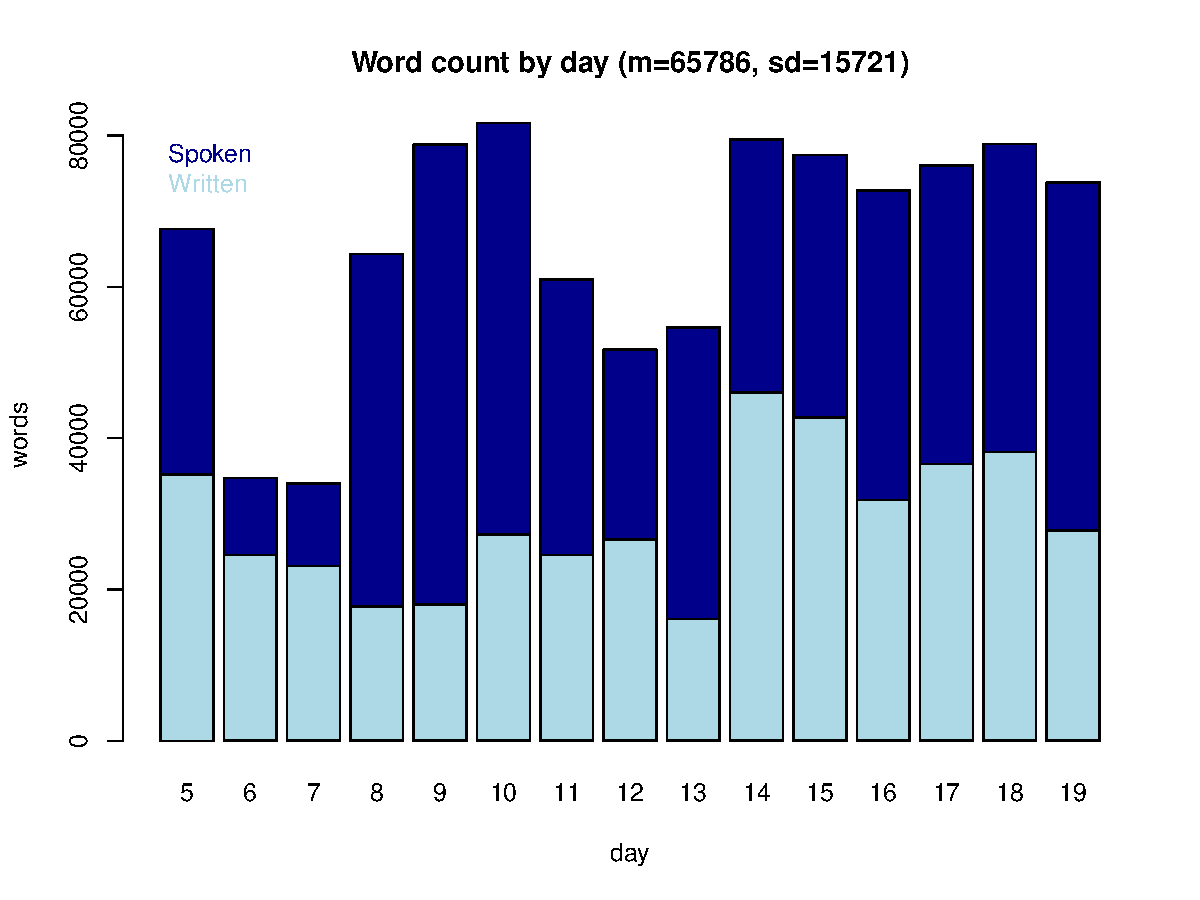
\includegraphics[width=0.8\textwidth]{cbyday}
\caption{Daily event frequencies}
\label{fig:personal:eventcountbyday}
\end{figure}


Figure~\ref{fig:personal:eventcountbyday} shows the number of events recorded each day.  It shows event counts between 124 and 969, with much of the variation being expressed in terms of written data.  \td{a large amount of that 969 is terminal stuff from developing lwac all day}.

Contrary to expectations, and in part due to large aomunts of terminal and web use during software development work, the majority of daily language use is written.  This is contrasted by Figure~\ref{fig:personal:wordcountbyday}, which indicates that spoken events are likely to expunge greater amounts of words in a single event (spoken median is 128 words, vs. 27 words for written).  This is largely explainable by a penchant for consuming broadcast media (especially spoken radio), which have large amounts of ongoing spoken content.

% > mean(dat[which(dat$mode == 's'),]$computed_words)
% [1] 307.464
% > mean(dat[which(dat$mode == 'w'),]$computed_words)
% [1] 76.68702
% > sd(dat[which(dat$mode == 's'),]$computed_words)
% [1] 938.2
% > sd(dat[which(dat$mode == 'w'),]$computed_words)
% [1] 196.6995
% 


\begin{figure}[p]
\centering
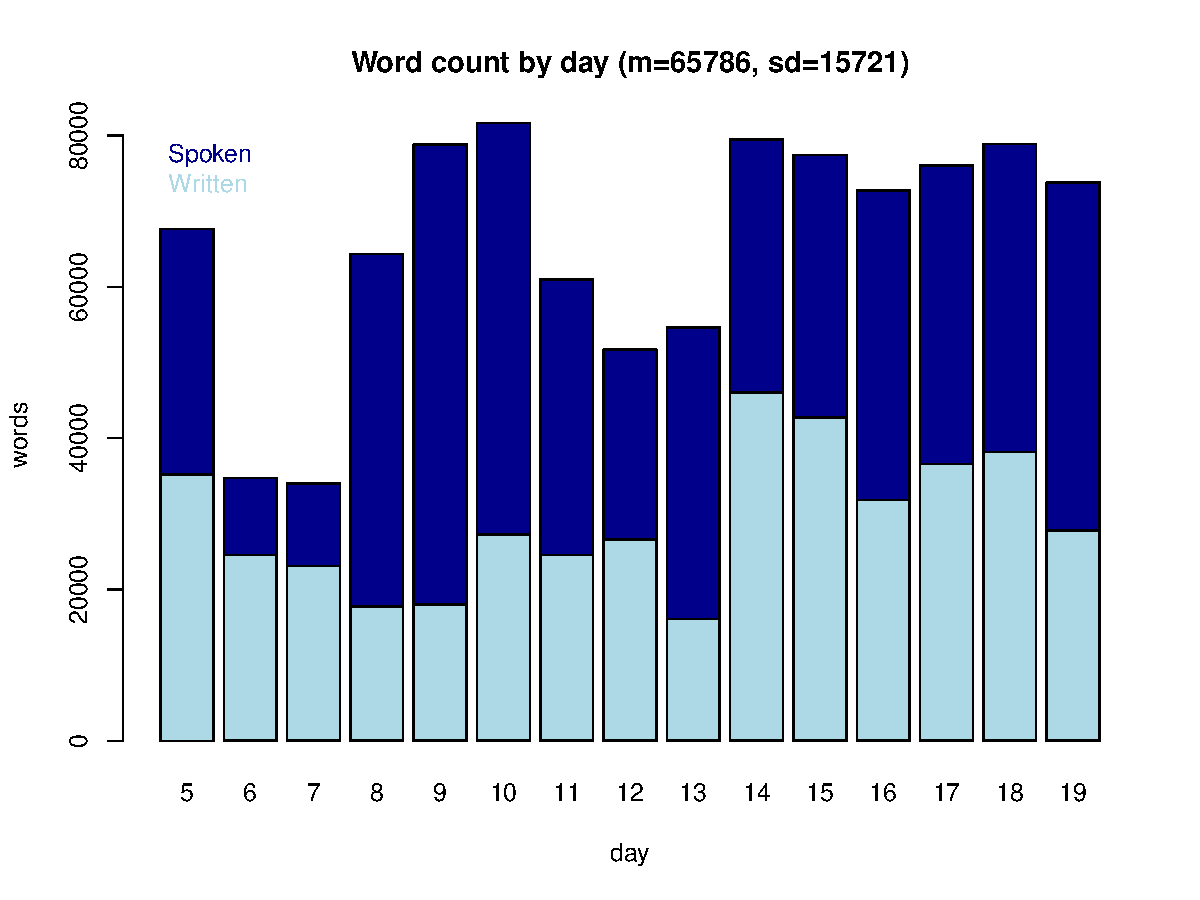
\includegraphics[width=0.8\textwidth]{cbyday}
\caption{Daily word counts}
\label{fig:personal:wordcountbyday}
\end{figure}

As shown in Figure~\ref{fig:personal:eventcountbyday}, the event count as broken down by day shows that between 35,000 and 80,000 words were used each day.  As we shall see later, this is mainly explainable by way of broadcast media and web page views.  It is notable that weekends fall upon days 6,7,13 and 14.  There is no significant pattern by day.

Before this study it was conjectured that the vast majority of all language used would be 



\til{More fun breakdowns, plot and comment on the distribution of some larger features throughout the data}





\subsubsection{Events}

\til{Plot event by source, bar plot}
\begin{figure}[p]
\centering
% 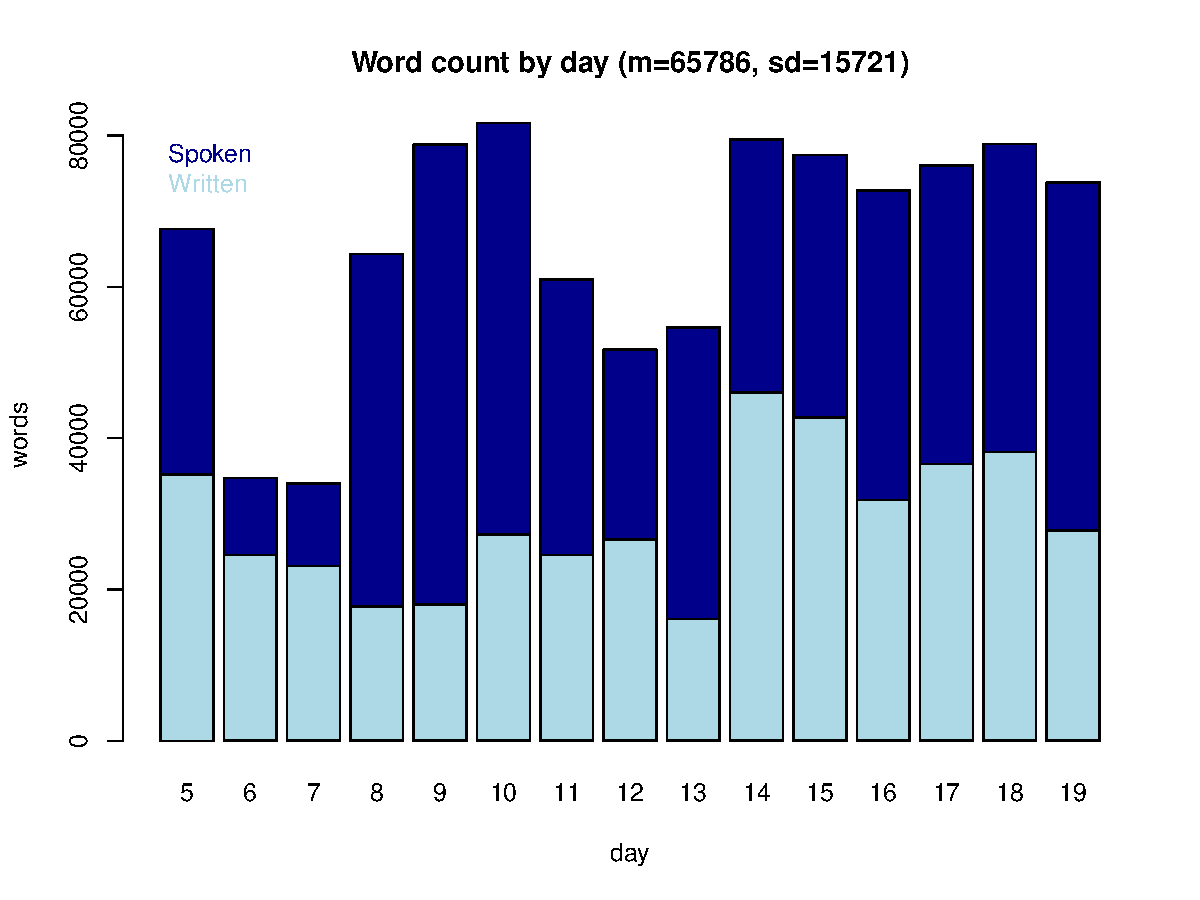
\includegraphics[width=0.8\textwidth]{cbyday}
\begin{verbatim}
    call    email     file      irc    music    notes   photos      sms 
      14      184      279      266     1433      272      152       28 
   squid terminal 
    6076     1214 
\end{verbatim}
\caption{Event count by source}
\label{fig:personal:eventsbysource}
\end{figure}

The proportions described in Figure~\ref{fig:personal:eventsbysource} are likely a very individual trait of the subject.  They exhibit a number of properties that would be significantly affected not only by daily routine, but also the specific work being completed at the time of the sample (the implications of this on scientific validity are discussed below in section~\ref{}\td{ref}).

Particularly curious is the large number of terminal, web (squid), and music events.  These are partially explainable by the work being completed at the time of the study, as the subject was developing software, listening to music whilst doing so and using many web references as documentation.  The subject also uses a GUI on his computer that mandates use of terminals for many tasks (this is doubtless atypical).



\begin{table}[ht]
\centering
\begin{tabular}{rr}
  \hline
  Computed Genre & Events \\ 
  \hline
  web/entertainment/social & 2598 \\ 
  web/music & 708 \\ 
  display/output & 627 \\ 
  music/punk & 587 \\ 
  web/reference & 421 \\ 
  web/shopping & 388 \\ 
  display/interactive & 285 \\ 
  web/academic & 280 \\ 
  web/tech & 218 \\ 
  web/outdoors & 180 \\ 
  web/video streaming & 167 \\ 
  irc/informal/discussion & 159 \\ 
  music/guitar & 147 \\ 
  web/academic/reference & 142 \\ 
  web/tech/reference & 116 \\ 
  web/news & 105 \\ 
  file/ruby code &  82 \\ 
  music/metal &  73 \\ 
  music/pop &  68 \\ 
  music/rock &  67 \\ 
  web/hosting &  54 \\ 
  file/documentation &  49 \\ 
  web/comedy &  49 \\ 
  web/social &  49 \\ 
  web/product support &  48 \\ 
  product/packaging &  43 \\ 
  web/tech/academic &  40 \\ 
  TV/comedy &  39 \\ 
  web/outdoors/reference &  36 \\ 
  email/academic &  34 \\ 
  email/advertising &  28 \\ 
  web/entertainment &  28 \\ 
  email/personal &  26 \\ 
  file/config &  24 \\ 
  email/business &  22 \\ 
  speech/discussion &  22 \\ 
  speech/informal &  21 \\ 
  web/comedy/social &  21 \\ 
  email/orders &  20 \\ 
  speech/service &  19 \\ 
  web/search &  19 \\ 
  email/spam &  17 \\ 
  music/blues &  17 \\ 
  speech/greeting &  16 \\ 
  web/fitness &  16 \\ 
  web/tech/news &  15 \\ 
  TV/Entertainment &  14 \\ 
  speech/info &  14 \\ 
  web/tech/shopping &  14 \\ 
  web/reference/academic &  13 \\ 
  TV/news &  12 \\ 
  radio/music &  12 \\ 
  radio/news &  12 \\ 
  sign/info &  11 \\ 
  web/art &  11 \\ 
  web/music/shopping &  11 \\ 
  music/folk/metal &   9 \\ 
  music/progressive &   9 \\ 
  TV/entertainment &   8 \\ 
  email/technical &   8 \\ 
  sign/info/instruction &   8 \\ 
  speech/ephemera &   8 \\ 
  web/banking &   8 \\ 
  music/country/rock &   7 \\ 
  music/fusion &   7 \\ 
  sign/product info &   7 \\ 
  book/info &   6 \\ 
  sign/advertising &   6 \\ 
  TV/documentary &   5 \\ 
  flyer/advertising &   5 \\ 
  notes/note &   5 \\ 
  product/info &   5 \\ 
  speech/parting &   5 \\ 
  web/advertising &   5 \\ 
  web/conspiracy &   5 \\ 
  box/address &   4 \\ 
  flyer/info/advertising &   4 \\ 
  radio/news/entertainment &   4 \\ 
  sms/informal &   4 \\ 
  web/blogs &   4 \\ 
  web/games &   4 \\ 
  web/news/social &   4 \\ 
  web/reference/social &   4 \\ 
  web/reference/travel &   4 \\ 
  web/reference/woodwork &   4 \\ 
  web/shopping/investment &   4 \\ 
  web/tech/utility &   4 \\ 
  web/utility &   4 \\ 
  TV/advertising &   3 \\ 
  application/info &   3 \\ 
  file/js code &   3 \\ 
  flyer/menu &   3 \\ 
  music/country &   3 \\ 
  phone/ &   3 \\ 
  sign/advertising/info &   3 \\ 
  sms/info &   3 \\ 
  speech/organisation &   3 \\ 
  speech/request &   3 \\ 
  web/health &   3 \\ 
  web/news/tech &   3 \\ 
  application/info/status &   2 \\ 
  book/packaging/book title &   2 \\ 
  map/info &   2 \\ 
  music/indie &   2 \\ 
  paper slip/invoice &   2 \\ 
  phone/informal &   2 \\ 
  poster/advertising &   2 \\ 
  radio/News &   2 \\ 
  speech/Discussion &   2 \\ 
  speech/informal/discussion &   2 \\ 
  web/comedy/entertainment &   2 \\ 
  web/entertainment/images &   2 \\ 
  web/entertainment/news &   2 \\ 
  web/entertainment/puzzles &   2 \\ 
  web/game &   2 \\ 
  web/tech/social &   2 \\ 
  TV/advertising/info &   1 \\ 
  TV/documentary/entertainment &   1 \\ 
  TV/info &   1 \\ 
  TV/music &   1 \\ 
  TV/sport &   1 \\ 
  application/album listing &   1 \\ 
  application/buttons/info &   1 \\ 
  application/update &   1 \\ 
  book/ &   1 \\ 
  book/packaging/book blurb &   1 \\ 
  box/packaging &   1 \\ 
  card/info &   1 \\ 
  cheque/info &   1 \\ 
  clothing/packaging &   1 \\ 
  display/info &   1 \\ 
  display/info/status &   1 \\ 
  file/html code &   1 \\ 
  film/Entertainment &   1 \\ 
  game/discussion &   1 \\ 
  game/game &   1 \\ 
  music/classical &   1 \\ 
  music/electronica &   1 \\ 
  music/music &   1 \\ 
  music/pop/metal &   1 \\ 
  notes/agenda/minutes &   1 \\ 
  notes/diagram &   1 \\ 
  noticeboard/advert &   1 \\ 
  paper slip/info &   1 \\ 
  phone/info &   1 \\ 
  poster/info &   1 \\ 
  poster/menu &   1 \\ 
  product/instruction/info/packaging &   1 \\ 
  radio/News/entertainment &   1 \\ 
  sign/ &   1 \\ 
  sign/instruction &   1 \\ 
  sign/map &   1 \\ 
  sign/menu &   1 \\ 
  sms/ &   1 \\ 
  speech/Informal &   1 \\ 
  speech/Inquiry &   1 \\ 
  speech/discussion/academic &   1 \\ 
  speech/info/discussion &   1 \\ 
  speech/question &   1 \\ 
  speech/service/discussion &   1 \\ 
  taxdisc/info &   1 \\ 
  vehicle/branding/sign &   1 \\ 
  vehicle/info/advertising &   1 \\ 
  video/info/academic &   1 \\ 
  video/info/advertising &   1 \\ 
  web/downloads &   1 \\ 
  web/games/news &   1 \\ 
  web/info/advert &   1 \\ 
  web/reference/entertainment &   1 \\ 
  web/reference/military &   1 \\ 
  web/reference/outdoors &   1 \\ 
  web/reference/shopping &   1 \\ 
  web/tech/hosting &   1 \\ 
   \hline
\end{tabular}
\caption{Event frequency by computed genre}
\label{table:personal:eventcountbygenre}
\end{table}


Table~\ref{table:personal:eventcountbygenre} shows a breakdown of event frequencies by computed genre \td{probably exclude hapaxes to shorten the table?} (which includes the source).  This shows a somewhat predictable zipfian distribution of genres surrounding a number of themes:

\begin{itemize}
    \item Daily events, such as reading social media websites
    \item Short events, such as consuming single programs of media (especially songs due to additive effects with the above)
    \item Any of the above that are particularly surrounding personal interests of the subject
\end{itemize}

Clearly, the last of these is the most obvious and desirable effect of building a corpus using this method.  The overwhelming prevalence of \texttt{web/entertainment/social} events may be explained (rather embarrassingly) by one website, which displays a single image per page (along with socially-contributed captions), and thus demands a lot of page reloads for relatively little content.





\subsubsection{Word Counts}

\begin{table}[ht]
\centering
\begin{tabular}{rrrrrrrr}
  \hline
 & 5\% & 10\% & 20\% & 50\% & 70\% & 90\% & 95\% \\ 
  \hline
1 & 0.00 & 0.00 & 8.90 & 27.85 & 74.00 & 217.00 & 354.88 \\ 
   \hline
\end{tabular}
\caption{Percentiles for words-per-event.}
\label{table:personal:wordsperevent}
\end{table}

Word counts were established either directly, or by assuming an 80 word-per-minute speech ratetd{cite where this figure was pulled from, mention that song lyric estimates also back it up}.  Table~\ref{table:personal:wordsperevent} shows that the distribution of word count per event is heavily skewed towards the lower end, with the median being 27 words per event.

This figure also reflects the degree to which the attention model affects results---disabling calculations for this, the distribution of word counts is affected significantly by the largest source of data, web pages, becoming 442 words.  Most pages are, even compared to other types of event in the corpus, read only partially (often graphical clues indicate which portions to read, especially since most people revisit websites more than they visit new ones).









\subsubsection{Comparisons}
% Comparisons against BNC for genres, word counts etc.  Also extract demographic info from BNC for more targeted comparison
At a large scale, there are some obvious differences between the personal corpus and the BNC's selection.

One of the most striking of these is the rate of broadcast media consumption, which forms a full 50\% of the subject's spoken word count, yet only 10\% of the BNC's.  There is a fair argument to say that many people of a similar age, who grew up surrounded by online streaming services and easy access to cheap receiving devices, will share this disparity.

A less compelling difference is exhibited between the rate of spoken conversations---our subject's spoken data was 20\% conversational, whereas the BNC contains 40\% conversational data (as a proportion of its spoken component).  The degree to which this applies to others is difficult to estimate, since (contrary to the verbiage of this thesis) the subject may simply be unusually laconic.



Arguments for the diversity of texts within corpora are driven only vaguely by the quantitative findings of this study due to its restricted inter-person relevance.  Nonetheless, some trends were identified which could reasonably be expected to extend to many others in a similar culture.

Inspecting the selection of genres yields a diversity not covered in many corpora.  Though notably the BNC is quite good at this, covering many brochures and other such texts\td{examples}, it hardly represents the amount of times thanks were exchanged for holding a door open, bottles, cans and other labels were read (particularly addresses on mail), or a tax disc was checked.  It would seem that a corpus purporting to cover a large population would be awash with weirder texts, especially as those less academic than the subject here are likely to have relatively higher proportions of them in their corpora.

A particularly compelling argument is made for the inclusion of song lyrics.  These are a large portion of the corpus collected here \td{how big}, and often spawn sayings, memes and linguistic affectations that can last decades in popular culture.  It's also notable that this is one of the easier things to sample and music use by the population is meticulously documented and studied by the industry already (often in publicly available lists).



The comparisons from my presentation are qualitative, so I have left them for the discussion.  I'll revisit this when more time is available for subsetting the BNC's data.


\til{Do some tests to establish the variability and compare that (hapax counts, sources, etc)}





% 
% \subsection{Specific RQs...}
% 
% \til{Notes suggest uses: 
% 
% * Stratified Comparison
% * Synchronic Comparison
% * Vocabulary estimation
% * 'learning rate' estimation for some features (learner corpus stuff)
% }
% 
% 
% \til{ Technical problems,
%     coding problems,
%     what did I read/not read?,
%     What proportions were missing/over/under represented,
% }
% 






\section{Discussion \& Reflection}
The quantitative data presented above are of limited utility to others, since the degree to which they describe the subject's life (rather than some general linguistic trend) is unknown.  Without further sampling, or detailed linguistic auxiliary data, we cannot begin to generalise from the above in a useful manner.

This does not mean, however, that we cannot reason rationally about how transferrable those results are---it is more unlikely that a member of the general population is a software developer than it is that they watch TV, or listen to radio 4 in the mornings.

Moreover, since the purpose of the study is to assess the viability of methods, these may be seen as significantly more transferrable than the data they have collected (this distinction is blurred significantly by the inclusion of a human interest model, however.)






\subsection{Method}
The process of gathering data itself was optimised for low intrusiveness, and largely proved practical to persue for long periods of time.

Maintenance of the on-line notebook was the major interruption in everyday language use, and this was gradually optimised to a shorthand format that demanded less time in the field, yet more annotation to extract data.  Where the subject is someone other than the analyst, the format of journals would need to be solidified ahead of time to ensure all properties are identifiable.

On reflection, the mnemonic effects of the notebook were most useful---the narrative they created placed all other data items in context, and the detailed notes in the nightly journal contribute to an episodic memory that aided the coding process.  Again, this process of reflection is unlikely to be made available to an analyst without explicit insertion of an interview phase where the two may meet to resolve possible misconceptions.

The nightly journal, whilst useful during the study as a place to write down easily-forgotten details of language events, was less useful than anticipated during analysis.  In reality, the richness of the narrative one quickly notes down of a night proved to be difficult to operationalise, meaning that it was largely of use only as auxiliary data to augment the on-line notebook's event-by-event format.

Some sources of data proved significantly easier to operationalise (and subsequently normalise into a workable format) than did others.  (The suitability of each will depend heavily on the form of data one is aiming for when deciding to use similar methods, however).

SQUID logs proved particularly difficult to process largely due to technical reasons, as extensive whitelists and multiple manual inspection phases were necessary to disregard advertising and AJAX requests.  A possible solution to this would be to rely on sampling of web data closer to where it is consumed, for example through the use of a browser plugin.

Initial plans were to use Voice Activity Detection (or full automated transcription) to estimate word counts from verbatim audio recordings.  In practice the diversity of unwanted noise effects (background noise, positioning of microphone, overheard conversations) rendered this practically impossible.  Even rudimentary VAD algorithms work with frequency detection strategies, and some were liable to detect things such as music as continuous speech.  \td{say more on this}



% ---
\paragraph{}
Of particular interest to the methodology is the inclusion of a human interest model in the processing stages.  Without this model, the data is changed to massively overestimate the word counts of many data sources (some more than others), and it is the opinion of the subject that the model improves the plausibility of data.  Generalising the method requires generalising this model or narrowing down the number of sources it must cover (either by using more selective data gathering methods or by restricting the scope of the sample).  

Each of the data sources mentioned is burdened with its own empirical concerns that must be considered when designing a human interest model, and the general solutions for many of these may be particularly complex.  For example, models for websites using large graphical elements as well as text must take into account Gestalt principles as well as models for humans as they read text, and the particular interests of the subject.

One way this problem may be solved is through detailed eludication of particular features and interests via a questionnaire or laboratory tasks in addition to the data gathering methods described here.  Clearly, though, relating these to a usefully-complex model of human interest will demand significant further research.




One of the larger challenges in gathering data from so many sources (and in so many forms) is the amount of work needed to operationalise it.  This was done both manually (in the case of complex data such as photographs and notebook entries) and automatically (for the majority of sources).  Often, some degree of manual correction or annotation was necessary even where automated processing was used.  These processing tools were bespoke, and would need to be generalised if the method is to become viable for use gathering further samples.



% ---
\paragraph{}
A number of questions were raised during the sampling period surrounding the limits of data that should be captured.  The solutions used were taken from the subject's own judgement of what constituted language `use' (since this case study is predicated upon recording that opinion), however, further work would be needed to establish answers to these in the general case.


The attention models used to narrow down input have already been mentioned, however, they apply at a very specific level---often, shorter texts such as signs, brands and labels would have particularly familiar or conventional text placements, styles, and shapes (some media, such as road signs, deliberately accentuate these features to aid recognition).  It is unclear at what point a text is `read' rather than just recognised in the periphery of one's vision.  The solution used in this study was one of internal vocalisation---if the text was recognised sufficient to repeat it mentally, it was classed as read.  This means it is often possible to say that a text source had just a few words read, when in fact a number of boilerplate features were skipped over because of their position and style.


An extension of this problem is one of re-reading texts that are being written.  The degree to which this occurs is likely extremely variable by person and task, however, it proves to be a particularly complex form of the above problem and is particularly hard to measure (or even subjectively assess).  In this case study no attempt was made to compensate for this effect.  Detailed study using some kind of attention measuring system (for example, eye tracking) may allow for deliberately using attention models over 1 (for word counts) or deliberate repetition of data in the final corpus.


The nature of the attention system used in this case study is also debatable.  The current method of using a coefficient works only for estimating word counts, and does not favour certain regions of the final data over others.  Additionally, it conflates two effects---that of reading only a small proportion of the source text, and that of paying little attention to the text (you may also consider using the text at the same time as another a third form).  Annotation of simultaneous events was fairly simple in the notebooks, however, estimation of the distribution of one's attention was done only at a low resolution (the codes used practically equate to ratios of 80/20, 50/50, 20/80, 100 with only a few exceptions).



\til{ Specific experiences from the process of gathering data (take from notes, which are detailed on this) }



Since the aim of this study was to assess genre proportions, significant amounts of effort were saved by not converting all sources into verbatim text.  This is largely an issue of post-processing, as many methods were digital and thus yielded verbatim text with ease and those that do not have well established transcription procedures.  Of particular note is the importance of being able to apply a regional attention model to extract (or weight) the most read portions of a text, something that (as noted above) was not attempted here due to a focus on proportions and word counts.






\subsection{Sampling Period \& Validity}
It seems clear both from personal reflection and examination of the data, which strongly favours certain work-related activities over others, that a two-week sampling period is hardly enough to represent even an individual's language use.

There are a number of obvious reasons for this, particularly egregious examples being:

\begin{itemize}
    \item Some language sources are usually read slowly, such as books read at bedtime.  A sampling period that covers an individual's various literary interests would have to be very long indeed.
    \item Life is strongly periodic, and though attempts were made to cover the weekly cycle of work and weekend, many events occur annually (either due to seasons or social convention).  There are no christmas songs in my corpus.
    \item Many more obscure items were represented only once in the corpus (such as advertising on vehicles or documentation on things such as legal forms).  These features may not be periodic but they are ultimately rare.
    \item A person's behaviour is likely to be `chunky', following one pattern for a time and then deviating suddenly (for example, during holidays or upon a job change).  Significant effort would have to be given to careful description of duration and circumstance in order to make confident generalisation from the data captured using this method.
\end{itemize}

It is my opinion that this method is up against two major challenges which must be balanced in order to achieve some degree of scientific validity.  The former of these is the difficulty of sampling in-the-field.  The more obtrusive a method, the higher quality data is going to be, however, the shorter any practical sampling period is likely to be.

Given the relative paucity of metadata within many general-purpose corpora and the periodic/temporal complexity of life, it seems reasonable to suggest that an ideal mix would be better formed from long-term (multi-year) samples using low-resolution sampling techniques.  This may entail, for example, discarding the on-line journals and manual photography in favour of automated life-log photography and a nightly journal only.

Following sufficient short-duration studies, it would be possible to be more confident in the results of longer-term, lower-resolution samples, as the areas with less uncertainty may be attended to less intrusively.







\subsection{Data and Comparisons}
Compare rationally to BNC and conjecture how representative various corpora are for me

As mentioned in the quantitative section above, there are some large differences between the corpus gathered here and the BNC (here used as an example general-purpose corpus that purports to cover the subject).  It is clear that a number of these are down to individual variation (the technical and musical genre bias), however, other disparities are of an altogether more ambiguous status.

The overall word count of the BNC, and other similar corpora, is called into question by the size of this corpus.  In two weeks, a single person used almost a million words whilst focusing heavily on just a few subjects and roles.  Given the sheer number of people within the British population, their demographic variability, and the dubious extent to which even these two weeks represents our subject's use of language accurately, it seems preposterous to suggest that a mere 100 million (or even billion) words would sufficiently represent language use for almost any purpose.


\til{probably some more...}









\section{Validity}
The design of this experiment is subject to a number of challenges to validity, and is presented in an explanatory context.

* The proportions used are estimated and based on my subjective opinion
* When something is formally `read' is based on my subjective opinion
* Generalisability is low to others
* Any inference drawn from comparison to other corpora can be done rationally only, as quantiative data does not exist on inter-person variability



\section{Ethics}
The increased resolution of data pertaining to a single individual renders the methods discussed here ethically sensitive.  This sensitivity is increased further if continuous recording of audio or video are used, though, as mentioned above, this data was not integrated into my analysis.

There are a number of arguments justifying covert research in the social sciences, and ...


Further, future developments in the methods described may use questionnaires or other less-invasive methods as sources of auxiliary data.  These would be targeted to a particular study design and need not cover the full set of language uses, mitigating any ethical concerns by limiting the descriptive power of the raw data itself.

A number of technical measures are also possible that may assist this issue---some of these have been developed by \td{who} working on the Machine Listening project, who irreversably scramble their audio recordings in such a way that VAD algorithms may still run.  A further option is streaming of data to a remote server, which can process, summarise, and discard data on-the-fly to prevent any possible information security breaches.











% ============================================================================
\section{Future Work}

In the long term, it is hoped that a greater understanding of the above may contribute to:

\begin{itemize}
    \item Methods for augmenting and rebalancing corpora using a questionnaire or other surrogate auxiliary data
    \item A greater understanding of variance in terms of the populations being studied
    \item 
\end{itemize}

From a sample of just one person, it is possible to use auxiliary data from existing sources to operationalise and reason about inter-person variability.  This may be done by cross-referencing a subject's demographic variables with those from an existing corpus, placing them in context and allowing comparison of his linguistic data to other groups (or to those within a given similarity).

This technique can also be used to impute data from partially-sampled sources, creating a personal corpus by re-weighting existing samples.

Unfortunately many existing corpora are unsuitable for this process due to the limited availability of metadata (something that is also an issue for those constructing ``informal'' subsets).

% ---
Methodologically, it is possible to generalise the data-gathering procedures mentioned in this case study either through reduction of the population covered (the technique used here in extremis), or reduction in the linguistic fields covered (the technique used more typically in special-purpose corpora).

Careful application of elitication strategies such as questionnaires or source-specific tools like web usage monitors may be able to produce sufficient auxiliary data to resample larger corpora, however, these methods would need justification from repeated studies such as the one described here (which sample directly).




% ============================================================================
\section{Summary\td{are conclusions suitable for a case study?}}
There are a number of methodological challenges that continue to prevent application of the methods described here to larger populations.  These are either due to the problems inherent in sampling varied data in the first place (digitising photographs or transcribing audio), or the processing required to transform data into a usable form (models of attention).

It is hoped that further work will be able to develop these methods in order to mitigate these issues, at least for certain applications.  However, the utility of these methods to the thesis is retained under less ambitious conditions of restricting a combinatino of the domain (for example, only sampling web histories or work-day language use) and the population (i.e. only people very similar to myself).

The practical issues encountered during sampling are largely minor, and modern portable technology proved decisive in making capture of hitherto-unseen (or at least widely ignored) sources of text possible in-the-field.  The census design lends an empirical justification to inclusion of these genres in larger general-purpose corpora, however, we are unable to formally generalise with confidence to demographics other than that of the subject covered.

Of particular note (and perhaps greatest generalisability) is the number of words used throughout the sampling period.  Almost a million words were used by a single individual over a two week period.  Since it is reasonable to deduce that this sampling is at best representative only of a normal working week for a single individual, it is rational to suppose that a corpus purporting to cover the whole population of a country demands a sample size far greater than many existing corpora.


This would seem to form an argument that it is simply not cost-effective to build a conventional general-purpose corpus large enough to represent large populations, suggesting that the focus should lie in those built for more specialist purposes, or those sampled non-probabilistically.  Here, the extreme size of web corpora may be well justified, so long as they can be shown to have been sampled rigorously.


Of interest to this thesis is the high level of detail that may be captured using this method.  The census design affords full coverage of a given area about which we may wish to generalise, and the detail it is possible to capture this way makes the data ideal as a `seed' for constructing larger corpora with comparable properties.  Application of these methods, as well as those using auxiliary data mentioned above, will hopefully render this sampling method a complementary one, to be added to the collection of existing corpus designs.





% 
% 
% 
% \section{--- --- ---}
% % 
% % \section{Intro/review stuff}
% % 
% % There is some discussion about the value of proportionality in corpus building.  The web makes this discussion particularly interesting, as the availability of pages online is different to those in general life (for any web user, a sizable subset).
% % 
% % Using the methods above, it should be possible to control for the proportions of language used in daily life, to construct a corpus from these that is both web-sourced (and hence easy to sample) and yet balanced to a given population.  This is, in effect, the goal of many special purpose corpora sampled online.
% % 
% \section{Methods for Proportional Selection Online}
% Many web-as-corpus tools make at best modest efforts to constrain their output.  There are a number of good reasons for this:
% 
% \paragraph{Metadata Availability}
% Many of the variables available for balancing data online are of limited applicabilty to many corpus objectives: consider, for example, the data attached to many web pages, which is typically limited to the HTTP headers, location, and immediate context.  Many users will combine knowledge about the world and intuitions regarding content to judge the genre, author, and many other salient properties---something that is beyond the scope of many WaC processing toolchains.
% 
% This has been adjusted for using various methods, such as:
% 
% \begin{itemize}
%     \item Selection of only certain top-level-domains (i.e. those for a given country)
%     \item Use of HTTP headers to identify language or location of servers (limited due to poor coverage of internationalisation technologies)
%     \item Use of metadata and non-content HTML body data (applicable only where services make a layout/content distinction)
%     \item Heuristics (such as keyword counting in various languages; suitable only for simple inferences)
% \end{itemize}
% 
% 
% \paragraph{Internal Variables}
% The problem of metadata availability is compounded further by the need to select documents without systematic linguistic bias (especially where general-purpose corpora are concerned).  Many available properties of web documents are essentially internal variables, and should not be used for sampling.
% 
% One method for controlling for this relies on seed terms, where a search engine will be used to find pages containing various collocations from a corpus.  This method is essentially a complex heuristic, and is reliant either on the principle that search engines will duplicate external variables by summary of the content they select, or that the content will be summarised from the original document and selected without bias by the search engine.  In practice this method proves fast, easy, and able to control (at least to some extent) for more complex characterisation than the coarse definitions covered by page metadata.  This method is boosted further by the existence of boilerlate/non-content text in pages, which may prove cause for selection without itself being content for the corpus.
% 
% \paragraph{Format Heterogeniety}
% The format of web data is particularly heterogeneous, and this poses significant problems with respect to selection of pages based on their layout or appearance.  Without further (arbitrary) restriction by corpus compilers, the only common interface data online is designed for is the human eye (and some content even violates this assumption\footnote{Such as large dumps of tables, or things like JSON and XML serialisation formats.  Largely it is assumed that these will be excluded from the corpus by design anyway}).  
% 
% This means that any use of boilerplate and data surrounding the content itself is severely limited by our capacity to codify and process such a distinction---something that is easy for a corpus with few sources, but difficult for larger ones sampling wider population of text.
% 
% \paragraph{Population Ambiguity}
% As mentioned in [the special edition on web as corpus], web corpora may be seen, strictly, as only representative of web content.  The extent to which this applies in practice is a matter of debate.
% 
% Those who spider the web, such as WebCorp and other services, offer corpora that are perhaps most closely tied to its layout and content---they do not make any efforts to (re-)balance their corpora in terms of other proportions, and subsequently end up with a natural representation of web data.
% 
% Users of techniques such as those mentioned above are able to apply weighted selection policies to correct for this, however, the extent to which this is capable of correcting for the web's idiosynchrasies is debatable---issues of presentation (``click here") and context are at play for which there is no alternative source of data online, and this necessarily limits the power of any methods for mitigating differences between `real life' and web corpora. % TODO: rephrase and shorten
% \til{More stuff, elucidate more especially on this point since it's pretty crucial to the narrative} 
% 
% % 
% % \section{Establishing Proportions of Strata}
% % The proportions of corpora have traditionally been established through a combination of experiment, debate, and reason.  This process has been well documented in the early corpora, \todo{ read up on some examples to include here}
% % 
% % 
% % As with most aspects of corpus construction, practical limitations necessarily restrict the selection and variety of data sources available.  This has conventionally led to selection from large pre-indexed resources such as library catalogues, publisher's records, and bestseller lists.  We may see this stratification of variables as being primarily governed by the proportional consumption of text types, measuring the population's socioeconomically-influenced consumption of text by the text's popularity.
% % 
% % This method is contrary to many other samples in social science, which seek primarily to control for a given socioeconomically-defined population.  In the case of text corpora, the reasoning behind this is doubtless often pragmatic: it is far cheaper and simpler to rely on existing indexes, and brings us one step closer to gathering actual real-world book statistics.  This decision, then, may be seen as a generally wise and productive one for corpus linguistics, as it has freed the field from the need to fund and maintain even larger projects akin to the British Household Panel Survey or cohort studies.
% % 
% % Nonetheless, there are a number of disadvantages associated with this selection of variables.  One of the most pronounced scientifically is the definition of population: selecting primarily in terms of textual variables leads us to define our population in such a way, something that leads to an ambiguity in the boundaries of representation for the corpus, and the limits of generalisability for any resultant conclusions.  This effects is especially pronounced for special-purpose corpora, about which generalisations must be qualified with much greater specificity.
% % 
% % Other disadvantages with this method surround the power socioeconomic annotation gives to those using corpus resources.  Often, simpler annotations derived from text-oriented variables are insufficient to drill-down into a ``Who uses what'' question format, something that may be crucial in reducing within-class variance to the point where many techniques are useful.
% % 
% % Another property obscured by description in terms of texts is the differentiation between text production/performance and reception.  This distinction is well noted in corpus documentation (going back to Brown... % TODO: quote
% % ), but, except in circumstances where the distinction is of particular interest, often compromised.  Designs for corpora including Brown and the BNC state that their aim is to sample a ``mix'' of the two, so as to represent language use for the population (this is one major reason they take into account the relative popularity of works when selecting texts).  The lack of detail in this method denies any detailed inquiry into the ratio of text production and consumption, and any analyses and insights that lead from this.  Simply put, selection of texts from text-centric central indexes obscures this distinction.
% % 
% % \til{It might be wise to expand this section to debate the difficulties in text selection proportionally.  Also mention Leech, review things like the Czech NC}
% % 
% % It's worth noting here that the approach taken for written resources often differs to that for spoken.  The transient nature of spoken language mandates capture during performance, meaning that little of it is indexed.  Many spoken corpora thus contain data that was gathered by the authors themselves, affording an opportunity to both describe and balance the socioeconomic variables first with little effort.
% % 
% % As such, many spoken corpora are primarily oriented around these variables (in addition to text-format ones), for example the BNC's section, LLC, etc.  \todo{find examples}
% 
% 
% 
% 
% 
% 
% 
% 
% % 
% % \til{ talk about this allowing us to go out into the field and re-examine language use with less interruption,
% %     the ability to get empirical data on text proportinoality,
% %     lack of a need for a central index,
% %     better population definition
% % }
% % 
% 
% 
% 
% 
% \section{Scope}
% The methods presented here are intended as an inspection of the issues that surround construction of personalised corpora, and should be seen as a first step towards the principles of building a ``socially balanced'' set of important variables across which to sample.  
% 
% 
% 
% 
% 
% 
% \til{What aspects are in common with typical fieldwork?
% 
% Why stop where I did?
% 
% How long to sample for? Why?
% 
% Data sources.
% }
% 
% 
% 
% 
% 
% 
% 
% 
% 
% % ============================================================================
% \section{Method}
% In order to best derive methods of data recording that were practical and well-suited to the lifestyle of the subject, experimental design proceeded in an iterative fashion.  Ultimately there were two formal preliminary data gathering stages, and after each of these a summary was written to alter the procedure for the next.
% 
% 
% 
% 
% 
% \til{What I did, like...
% Should I describe the first preliminary approach as an iterative things?
% }
% 
% \subsection{Variable Selection}
% Variables selected for recording in the preliminary study were selected to be in line with those most commonly included in general-purpose corpora.  The decision was made to limit the number of these variables to facilitate unobtrusive recording (and maximise the relevance to the many different media recorded).
% 
% 
% 
% \til{Which variables I have tried to record and why}
% 
% 
% \subsection{Capture Methods}
% \til{ \\paragraph{}-ised list of methods }
% 
% 
% 
% \subsection{Annotation Methods}
% Corpus items were annotated along a small subset of the variables usually included in general purpose corpus metadata.  This was guided both by the practical concerns of the process and the literature % CITE atkins, clear, ostler
% .
% 
% In many cases there was a need to review and augment a text's main properties from memory and free-form notes.  This was done partially to reduce the intrusiveness of the initial recording process (which must be done as soon as possible after the text consumption event).  As such, though much metadata is available from inspection of pictures, recordings etc., some detailed properties (such as the country of origin of authors) are absent.  This was a deliberate design choice, as increased intrusivity of recording methods would have led to the exclusion of many minor linguistic events (a group most likely to be neglected using other methods of sampling).
% 
% 
% \til{Show initial intent, resultant listing, interpolation}
% 
% \section{Results}
% \til{ Perhaps move this section, but provide layouts}
% 
% \section{Discussion}
% 
% 
% 



